\apendice{Plan de Proyecto Software}

\section{Introducción}
Es esencial realizar al inicio de cada proyecto una planificación temporal del desarrollo del mismo, un presupuesto estimado del coste que va a suponer y un análisis de la normativa vigente que afecta a la viabilidad del mismo en el territorio correspondiente. Para ello se detallan en el presente anexo 3 secciones relativas a estas planificaciones.

\section{Planificación temporal}
La evolución del proyecto fue documentada mediante la utilización de GitHub, aplicación en la cual se definieron 6 milestones u objetivos principales del desarrollo del proyecto. Algunos de estos milestones se dividieron en diferentes issues:
\begin{itemize}
    \item Desarrollo de aplicación web
    \begin{itemize}
        \item Generación de informe descargable (incluye generación de gráficas básicas sobre las actividades)
        \item Personalización de tiempo de bloqueo (parte 1 y parte 2)
        \item Creación de un diario de fluctuaciones motoras
        \item Almacenamiento de datos del diario en la base de datos
        \item Registro de fecha y hora de las actividades realizadas
        \item Creación de gráficas que relacionen las fluctuaciones motoras con la toma de medicaciones y los bloqueos/min en actividades.
        \item Desarrollo front-end para el acceso a nuevas funciones desde la página web
    \end{itemize}
    \item Configuración del hardware
    \begin{itemize}
        \item Diseño de hardware nuevo
        \item Creación de nuevo hardware
        \item Pruebas de hardware
        \item Inserción de hardware en soporte flexible
    \end{itemize}
    \item Actualizaciones del código Arduino
    \begin{itemize}
        \item Adaptación del código Arduino al módulo láser
        \item Corrección del registro de duración total de las actividades
    \end{itemize}
    \item Redacción de memoria del proyecto: Este milstone abarca la redacción de los diferentes apartados de la memoria: Introducción, objetivos, conceptos teóricos, metodología, conclusiones y líneas futuras.
    \item Redacción de Anexos: Este milestone abarca la redacción de los diferentes Anexos (Anexo A- Anexo H).
    \item Elaboración de presentación para la defensa del proyecto
\end{itemize}
Debido a la naturaleza de la metodología iterativa utilizada, el cumplimiento de estos objetivos generales se realizó de forma simultánea a lo largo del desarrollo del proyecto. Los cambios en el código fueron actualizados en la plataforma Github mediante el software Github Desktop, mientras que los documentos redactados fueron redactados a lo largo del desarrollo del proyecto e incluidos en el repositorio al final del mismo.

El cumplimiento de cada tarea que compone los diferentes objetivos se planificó de manera inicial mediante el desarrollo del diagrama de Gantt mostrado en la figura \ref{fig:Diagramagantt}. Sin embargo, el cumplimiento real de esta planificación se refleja en el diagrama de Gantt mostrado en la figura \ref{fig:Diagramagantt2}.

\begin{sidewaysfigure}
    \centering
    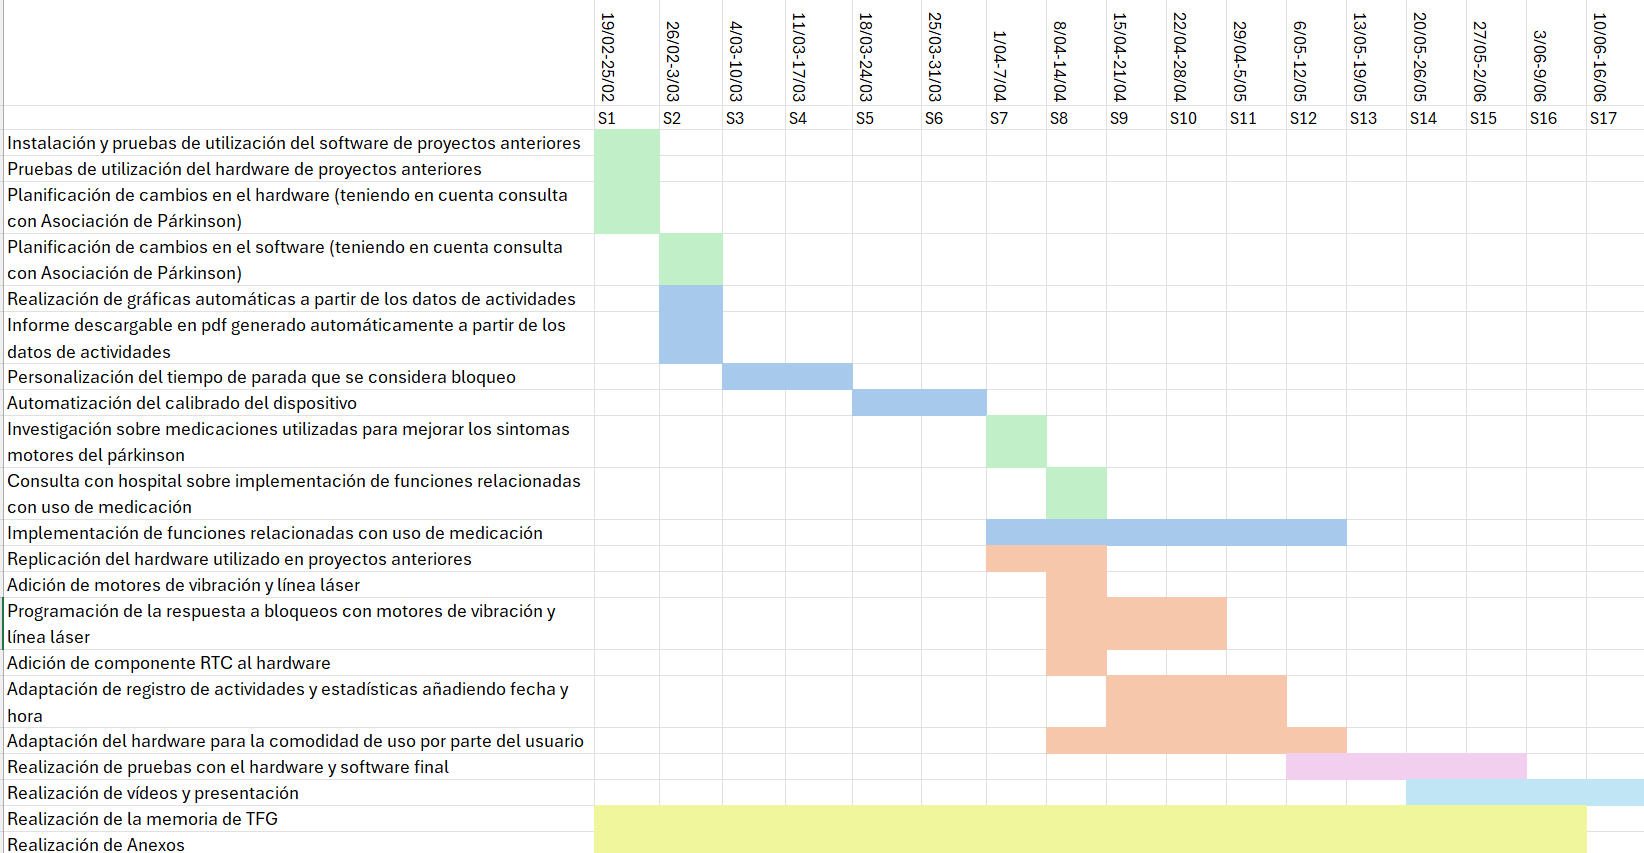
\includegraphics[width=1\textwidth]{img/gant1.png}
    \caption{Diagrama de Gantt: planificación temporal inicial del proyecto}
    \label{fig:Diagramagantt}
\end{sidewaysfigure}

\begin{sidewaysfigure}
    \centering
    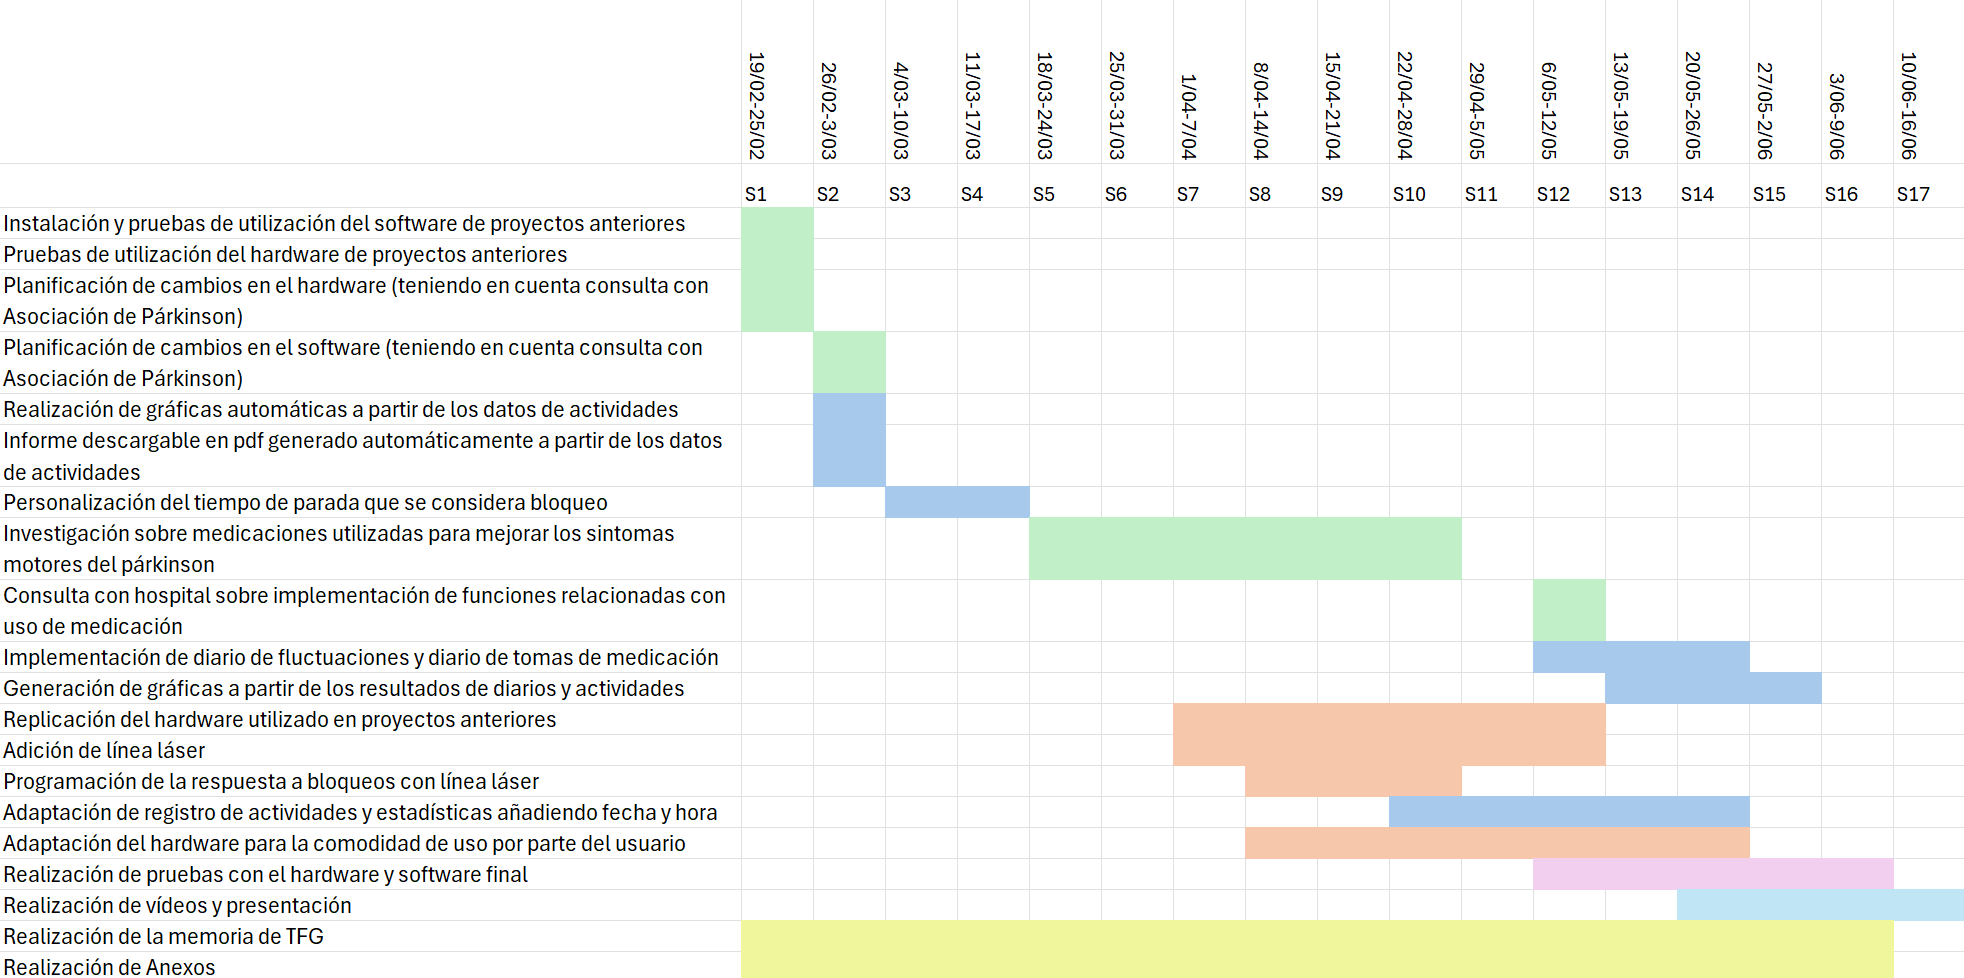
\includegraphics[width=1\textwidth]{img/gant2.png}
    \caption{Diagrama de Gantt: planificación temporal final del proyecto}
    \label{fig:Diagramagantt2}
\end{sidewaysfigure}

\section{Planificación económica}
El coste total de el proyecto, incluyendo costes de personal, software, hardware, amortización del ordenador utilizado y materiales es de aproximadamente 4982.3 euros. A continuación se describen en detalle cada uno de estos costes.
\subsection{Costes de personal}
El sueldo medio del ingeniero biomédico junior (con 0 a 3 años de experiencia) en España es de 29.020 € brutos por año \cite{jobted-ingeniero-biomedico}. Las horas empleadas en la realización del proyecto son equivalentes a 4 meses de trabajo con jornada parcial o 2 meses a jornada completa. Esto hace que el coste de personal durante la realización del proyecto sea de unos 4836,7€ brutos.
\subsection{Costes del software utilizado}
El software utilizado fue de código abierto, gratuito o facilitado con los paquetes disponibles para estudiantes de la Universidad de Burgos, por lo que el proyecto no presentó costes de software. A continuación se desglosa la naturaleza de las herramientas software utilizadas (descritas en el apartado 'Metodología' de la memoria de este proyecto) y el motivo de la gratuidad de su uso:
\begin{itemize}
    \item XAMPP: software de código abierto, licencia Apache 2.0: uso, modificación y redistribución gratuitos.
    \item Visual Studio Code: software gratuito con licencia MIT: gratuito para su uso y distribución. 
    \item IDE Arduino: software de código abierto  con licencia GNU LPGL (Lesser General Public License): gratuito para su uso y redistribución, con libertad para modificar el código fuente.
    \item Autodesk Sketchbook: versión gratuita para el uso personal y educativo.
    \item Microsoft Visio y Microsoft Excel: Incluidos en el paquete de Microsoft 365 ofrecido de forma gratuita a los estudiantes de la Universidad de Burgos.
    \item Versión 2 de ChatGPT: uso gratuito, sujeto a los términos y condiciones de OpenAI.
    \item Lucidchart: Versión gratuita con funciones limitadas.
    \item Balsamiq Wireframes: Software comercial que requiere licencia de compra o suscripción para su uso. Se utilizó la prueba gratuita del mismo.
    \item Visual Paradigm: Versión gratuita para uso personal y académico.
    \item Tinkercad: Versión gratuita para uso personal, educativo y comercial (este último siguiendo los términos de servicio de Autodesk).
\end{itemize}
\subsubsection{Costes del hardware y materiales utilizados}

En la tabla \ref{tab:preciomateriales} se desglosa el coste de cada material y herramienta hardware utilizados en el proyecto. El coste total de estos materiales supone 89.8 euros para la construcción de un prototipo.


\begin{table}[]
\begin{tabular}{
>{\columncolor[HTML]{DAE8FC}}l 
>{\columncolor[HTML]{EFEFEF}}l }
\cellcolor[HTML]{C0D5E5}Material/hardware & \cellcolor[HTML]{C0D5E5}Precio \\
Microcontrolador Arduino UNO R3           & 28 euros                       \\
Sensor MPU-6050                           & 5.99 euros                     \\
Pantalla LCD 16x2 con módulo LCD I2C      & 4.99 euros                     \\
2 pulsadores                              & 0.06 euros                     \\
Módulo láser                              & 4.99 euros                     \\
Módulo bluetooth HC-05                    & 9.99 euros                     \\
Interruptor ON/OFF                        & 3.99 euros                     \\
Conector aviación 4 pines                 & 1.77 euros                     \\
1m Cable multihilo 4 núcleos              & 2.39 euros                     \\
2m cable                                  & 0.42 euros                     \\
Fuente de alimentación recargable 9V      & 9.99 euros                     \\
Miniplaca de pruebas para Arduino         & 1.33 euros                     \\
Cable adaptador de batería Arduino DC 9V  & 3.90 euros                     \\
Riñonera/cinturón deportivo               & 11.99 euros                   
\end{tabular}
\label{tab:preciomateriales}
\caption{Desglose de los costes de materiales y hardware}
\end{table}

\subsection{Amortización de los equipos}
Se ha utilizado un dispositivo LG Gram 17ZD90R Intel Core i7-1360P/16GB. El coste de este dispositivo ha sido de 1172€, y se estima una vida útil de 7 años.
La amortización lineal de un producto puede estimarse mediante la siguiente fórmula \cite{liberto2024straightline}:

\text{Amortización lineal} = (\text{Precio de Compra del Activo} - \text{Valor Residual})/ \text{Vida Útil Estimada del Activo}

Con el objetivo de calcular la amortización lineal mensual del dispositivo utilizado, se utiliza por tanto la siguiente fórmula:

\text{Amortización lineal mensual} = (\text{Precio de Compra del Activo} - \text{Valor Residual})/ \text{Vida Útil Estimada del Activo en meses}

\text{Amortización lineal mensual} = (\text{1172€} - \text{0€})/84 \text{ meses} = \text{13,95€/mes}

Se calculará la amortización lineal del dispositivo en un periodo de tiempo de 4 meses:

\text{Amortización lineal total} = \text{13.95€/mes}* \text{4 meses}= 55.8€

\subsection{Viabilidad legal}
Con el objetivo de garantizar el cumplimiento del proyecto con las normas establecidas para dispositivos médicos y aplicaciones relacionadas con la salud en España, es importante tener en cuenta una serie de normativas a nivel europeo y nacional relacionadas con la comercialización de dispositivos médicos y la protección de datos, las cuales se exponen a continuación:
\subsubsection{Comercialización de dispositivos médicos}
Acorde con el Reglamento (UE) 2017/745 \cite{reglamento-ue-2017-745}, tanto la aplicación web como el dispositivo presentados en el presente proyecto entran dentro de la categoría de productos sanitarios. Este reglamento clasifica los dispositivos médicos en diferentes clases según su riesgo, requiriendo los dispositivos pertenecientes a cada clase diferentes procedimientos para la evaluación de conformidad. 

El presente dispositivo pertenercería a la clase I o clase de riesgo bajo, compuesta por los dispositivos que no están en contacto invasivo con el cuerpo o tan sólo están en contacto externo con la piel intacta, como es el caso del dispositivo presentado. Pertenecer a esta clase simplifica significativamente el proceso de comercialización, permitiendo por ejemplo la auto-certificación del dispositivo. Sin embargo, son obligatorios el cumplimiento de unos requisitos.

Uno de estos requisitos es el marcado de Conformidad Europea (CE), de obligado cumplimiento para todos los dispositivos médicos a comercializar dentro de la Unión Europea.

El Real Decreto 192/2023 \cite{BOE-A-2023-7416} en relación con la comercialización y puesta en servicio de productos sanitarios regula el registro, etiquetado y trazabilidad de estos productos en España. Este Real Decreto dicta que los agentes que comercialicen estos productos deben registrarse en la Agencia Española de Medicamentos y Productos Sanitarios, actualizando anualmente su información y manteniendo registros sobre sus productos y movimientos de los mismos.
\subsubsection{Protección de datos personales}
El Reglamento General de Protección de Datos (RGPD) (Reglamento (UE) 2016/679) \cite{reglamento-ue-2016-679} establece una serie de condiciones para el tratamiento de datos personales en la Unión Europea. Estas condiciones son la obtención de consentimiento explícito, la implementación de medidas que garanticen la seguridad de los datos personales y otorgar una serie de derechos a los sujetos cuyos datos se están utilizando sobre estos datos, como el acceso, rectificación, portabilidad o supresión de los mismos.

La Ley Orgánica 3/2018 de Protección de Datos Personales y garantía de los derechos digitales (LOPDGDD) \cite{ley-organica-3-2018} adapta el Reglamento General de Protección de Datos (RGPD) al contexto español, proporcionando detalles sobre la aplicación del mismo.